\documentclass[prd,aps,letter,twocolumn,floatfix,notitlepage]{revtex4-1}

%% packages
\usepackage{graphicx,psfrag}
\usepackage{mathrsfs,amsmath,amsfonts,amssymb, bm}
\usepackage{multirow}
\usepackage{comment,hyperref}
\usepackage{float}
\usepackage{algorithm}
\usepackage{algpseudocode} % in place of algorithmic. Conflicts with revtex4 unless [H] option passed
\usepackage{setspace} % for pleasent spacing in algorithm
\usepackage{times}

%% macros
\newcommand{\be}{\begin{equation}}
\newcommand{\ee}{\end{equation}}
\newcommand{\bsube}{\begin{subequations}}
\newcommand{\esube}{\end{subequations}}

\def\l{\ell}
\def\blambda{{\bm \lambda}}
\def\bLambda{{\bm \Lambda}}
\def\blam{\bar{\lambda}}
\def\Lam{\Lambda}
\def\Lamt{\tilde{\Lambda}}
\def\dLamt{\tilde{\delta{\Lambda}}}
\def\bmu{{\bm \mu}}
\def\btheta{{\bm \theta}}

%% macros for comments
\usepackage{color}
%% colors
\definecolor{cyan}{rgb}{0,0.9,0.9}
\definecolor{orange}{rgb}{0.9,0.5,0}
\definecolor{magenta}{rgb}{1,0,1}
\definecolor{purple}{rgb}{0.8,0.4,0.8}
\definecolor{gray}{rgb}{0.8242,0.8242,0.8242}
%%
\newcommand{\bs}[1]{{\textcolor{green}{\texttt{SB: #1}} }}
\newcommand{\bl}[1]{{\textcolor{blue}{\texttt{BL: #1}} }}
\newcommand{\cg}[1]{{\textcolor{orange}{{CG: #1}} }}
\newcommand{\cvdb}[1]{{\textcolor{purple}{\texttt{CVDB: #1}} }}
\newcommand{\red}[1]{\textcolor{red}{#1}}
%% +++++++++++++++++++++++++++++++++++++++++++++++++++++++
\begin{document}

\title{Surrogate model for aligned-spin binary neutron star waveforms using gaussian process regression}

\author{
Benjamin D. Lackey$^1$, 
Michael P\"{u}rrer$^1$
Andrea Taracchini$^1$
}
\affiliation{
$^1$Max Planck Institute for Gravitational Physics, Albert Einstein Institute, D-14476 Golm, Germany
} 

\date{\today}

\begin{abstract}

Construct 5d hierarchical surrogate model using reduced bases and GPR. Includes $\ell=2,3,4$, dynamical tides, 
and tapering fit to NR.

Provide framework for building high dimensional surrogate from NR.


\end{abstract}

\pacs{
  % 04.25.D-,   % numerical relativity
  % 
  04.30.Db,   % gravitational wave generation and sources
  % 04.40.Dg,   % Relativistic stars: structure, stability, and oscillations
  % 04.70.Bw,   % classical black holes
  95.30.Sf,     % relativity and gravitation
  % 
  % 95.30.Lz,   % Hydrodynamics
  % 97.60.Jd    % Neutron stars
  % 97.60.Lf    % black holes (astrophysics)
  % 98.62.Mw    % Infall, accretion, and accretion disks
}

%%
\maketitle

%% Template for figures
%% \begin{figure}[t]
%%   \centering 
%%     \includegraphics[width=0.49\textwidth]{../fig/ }
%%     \caption{ }
%%  \label{fig: }
%% \end{figure}

%% Template for tables
%% \begin{table}[t]
%%   \centering    
%%   \caption{ }
%%   \begin{tabular}{ccc}        
%%     \hline
%%     col$1$ & col$2$ & col$3$ \\
%%     \hline
%%     &  &  \\
%%     \hline
%%   \end{tabular}
%%  \label{tab: }
%% \end{table}


\red{Change arrow vectors to bold vectors. ${\bm x}^i$ (bold) for example $i$. $x_j$ (not bold) for coordinate/parameter/feature $j$. 
$x_j^i$ (not bold) for feature $j$ of example $i$.}


%% ________________________________________________________
\section{Introduction}



We organize the paper as follows. In Section...

\textit{Conventions:} Unless explicitly stated, we use units where $G=c=1$. To agree with the machine learning literature, we will refer to the waveform parameters (features) as $\vec x$ and the hyperparameters in the Gaussian Process Regression model as $\vec\theta$.

%% ________________________________________________________
\section{Aligned-spin, dynamical tides EOB model}
Ever since its inception~\cite{Buonanno:1998gg}, the effective-one-body (EOB) approach to the general-relativistic 2-body problem has proven successful in modeling the dynamics and GW emission of binaries of compact objects. State-of-the-art aligned-spin EOB models~\cite{Bohe:2016gbl,Nagar:2017jdw} can accurately match numerical-relativity (NR) simulations of spinning, nonprecessing binary black holes (BBHs) for mass ratios up to 8 and spin magnitudes up to 0.85 for unequal-mass (up to almost extremal for equal-mass) binaries. The EOB framework can also accommodate precessing-spin BBHs, showing good agreement to mildly precessing NR simulations~\cite{Babak:2016tgq}. This research program has been extended to accommodate matter effects~\cite{}, which become relevant XXX

References~\cite{Hinderer:2016eia,Steinhoff:2016rfi} built upon the aligned-spin BBH EOB model of Ref.~\cite{Taracchini:2013rva} and proposed a way to include the effect of dynamical tides. Neutron stars that are part of a compact-object binary will deform in the tidal field generated by the companion --- be it a black hole or another neutron star. Because of binary motion, the forcing tidal field varies at the orbital frequency. Thus, in the late stages of the inspiral, the characteristic $f$-mode frequency of the neutron star can be dynamically approached, resulting in a resonant excitation of such mode. The net effect is an amplification of tidal effects as compared to the adiabatic limit, which assumes that the $f$-mode frequency is much larger than the frequency of the forcing tidal field. Dynamical tidal effects are implemented in the EOB model through a modification of the radial potential $\Delta_u$, which is the $tt$-component of the metric of the effective spacetime. Here we adopt the tidally-augmented expression of $\Delta_u$ that is discussed in Appendix~A of Ref.~\cite{Steinhoff:2016rfi}, namely
\begin{equation}
\Delta_u = \Delta_u^{\textrm{pm}} + \Delta_u^{\textrm{DT}}\,,
\end{equation}
where $\Delta_u^{\textrm{pm}}$ is the 4PN-accurate point-mass term of the underlying BBH EOB model of Ref.~\cite{Bohe:2016gbl} (see Eq.~(2.2) therein) and $\Delta_u^{\textrm{DT}}$ is the contribution due to dynamical tides. We consider the general case of a binary that may consist of two neutron stars; if either component of the binary is a black hole, then vanishing values of the tidal polarizabilities are employed in the formulas below. Let $A$ and $B$ be the body labels. Let $M^{A,B}$ be the mass of either body and $M=M^A+M^B$ be the total mass of the binary.  Explicitly, including quadrupolar and octupolar tidal effects, we have
\begin{widetext}
\begin{align}
 \Delta_u^{\textrm{DT}} =&  - 3\,\Lambda_{2,\textrm{dyn}}^{A}(u)\,u^6\frac{X_B}{X_A} \left[ 1 + \frac{5}{2} X_Au + \left(3 + \frac{1}{8}X_A + \frac{337}{28} X_A^2\right)u^2 \right]\nonumber\\
 &- 15\,\Lambda_{3,\textrm{dyn}}^{A}(u)\,u^8 \frac{X_B}{X_A}\left[1 + \left(-2 + \frac{15}{2}X_A\right)u + \left(\frac{8}{3} - \frac{311}{24}X_A + \frac{110}{3}X_A^2\right) u^2\right] + (A \leftrightarrow B)\,,
\end{align}
\end{widetext}
where $X_{A,B}=M^{A,B}/M$, $u=1/r$ is the inverse of the ($M$-rescaled) EOB radial coordinate, $\Lambda_{2,\textrm{dyn}}^{A,B}(u)$ are the dimensionless quadrupolar dynamical tidal polarizabilities, and $\Lambda_{3,\textrm{dyn}}^{A,B}(u)$ are the dimensionless octupolar dynamical tidal polarizabilities. Within the dynamical tides model, the tidal polarizabilities are not constant, but rather depend on the orbital separation and on the values of the $f$-mode frequencies. In particular, the dimensionless dynamical polarizabilities read
\begin{equation}
\Lambda_{\ell,\textrm{dyn}}^{A,B}(u)=\frac{2}{(2\ell-1)!!}k^{A,B}_{\ell}\hat{k}^{A,B}_{\ell\,\textrm{dyn}}(u;\omega_{0\ell}^{A,B})\left(\frac{R_{A,B}}{M}\right)^{2\ell+1}\,,
\end{equation}
where $k^{A,B}_{\ell}$ is the tidal Love number and $R_{A,B}$ is the neutron star radius. Here $\hat{k}^{A,B}_{\ell\,\textrm{dyn}}(u;\omega_{0\ell}^{A,B})$ is the separation-dependent, dimensionless enhancement factor given in Eq.~(11) of Ref.~\cite{Dietrich:2017feu}, which depends on the value of the $f$-mode angular frequency of the $2^\ell$-th multipole, $\omega_{0\ell}^{A,B}$. 

Tidal effects also enter the dissipative part of the model. In particular, the point-mass $\ell=2,3$ inspiral-plunge waveform modes are corrected by tidal terms
\begin{equation}
h_{\ell m}^{\textrm{insp-plunge}} = h_{\ell m}^{\textrm{insp-plunge, pm}} + h_{\ell m}^{\textrm{tidal}}\,,
\end{equation} 
where $h_{\ell m}^{\textrm{insp-plunge, pm}}$ is discussed in Section~II.B of Ref.~\cite{Bohe:2016gbl} and $h_{\ell m}^{\textrm{tidal}}$ is given by Eqs. (A14)-(A17) of Ref.~\cite{Damour:2012yf}. Following Ref.~\cite{Dietrich:2017feu}, in the computation of $h_{22}^{\textrm{tidal}}$ we include a dynamical enhancement factor that depends on the orbital separation and on the $f$-mode frequency, and is given in Eq.~(15) of Ref.~\cite{Dietrich:2017feu}.\red{[Tanja should confirm for 21]}


--Total mass is scaled out. This is fine, even up to zero amplitude point. Estimate the error in this approximation.

--Tapering fit to NR.

--Universal relations to relate all matter parameters to quadrupolar $\Lambda$.

--Results in 5 waveform parameters $\vec x=\{q, S_1, S_2, \Lambda_1, \Lambda_2\}$.

%% ________________________________________________________
\section{Evaluating waveform model accuracy}

In the sections below, we will use several criteria to choose waveforms samples and evaluate the accuracy of the 
surrogate waveform model. We briefly discuss them here.

--Phase error. (needs to be significantly smaller than tidal effects) Use this for order of magnitude estimate of required
accuracy.

--distinguishability

--Mismatch

As another common measure of the surrogate model accuracy, we examine the mismatch between 
the surrogate model and the original EOB waveform.
The mismatch represents the loss in signal-to-noise ratio that would result 
from using the surrogate model instead of the original EOB waveform. 
It is defined by the deviation from a perfect overlap after aligning the two waveforms
using the time and phase free parameters $t_0$ and $\phi_0$:
\begin{equation}
\mathcal{M} = 1 - \max_{t_0, \phi_0} \frac{(h_{\rm EOB}, h_{\rm Sur})} {\sqrt{(h_{\rm EOB}, h_{\rm EOB}) (h_{\rm Sur}, h_{\rm Sur})}}.
\end{equation}
The inner product here  is the integral of the Fourier transformed waveforms $\tilde h(f)$ weighted by the noise power spectral 
density (PSD) $S_n(f)$ of the detector:
\begin{equation}
(h_1, h_2) = 4 \Re \int_{f_{\rm low}}^{f_{\rm high}} \frac{\tilde h_1(f) \tilde h^*_2(f)} {S_n(f)} df.
\end{equation}

--Fisher matrix systematic error. (See spin NSBH paper.)

%% ________________________________________________________
\section{Surrogate model}

The problem of constructing a surrogate model for a computer simulation that takes parameters 
$\vec x$ and outputs a vector of data $\vec y$ is the following: construct approximate functions $f_j(x)$
for each quantity $y_j$ using a training set of precomputed examples $\{\vec x^i, \vec y^i\}$. For the problem here, 
our parameters are the intrinsic waveform parameters $\vec x$ and the data is the waveform frequency series $\tilde h(f_j)$. 

--Frequency-domain so Fourier transform can be done offline and all issues related to tapering, etc. are taken care of.

We aim to construct a sufficiently accurate waveform surrogate using as few waveform evaluations as possible.
To do this we perform the following steps:
\begin{enumerate}
\item Select the initial training set parameters.

\item Precondition an initial training set of waveforms, and decompose them into functions that smoothly vary
as a function of waveform parameters $\vec x$. 

\item Compress the waveform output using a greedy method for generating a reduced orthonormal basis and 
generate empirical interpolating functions and nodes form this reduced space, to minimize the number of interpolations
required.

\item Interpolate the waveform at the empirical nodes as a function of the waveform parameters $\vec x$ using GPR.

\item With the resulting surrogate model and GPR uncertainty estimate, perform uncertainty sampling to choose the 
next waveforms to add to the training set.

\item Repeat steps 2--5 to reconstruct the surrogate model with the updated training set. This can be repeated
if necessary.
\end{enumerate}

\subsection{Initial training set design}

In constructing a surrogate model, we will need to interpolate several quantities as a function of the five
waveform parameters ${\bm x}$.
Most multivariate interpolation techniques (e.g. tensor spline or Chebyshev interpolation) 
require a function to be sampled on a rectangular grid, and thus suffer from the curse of dimensionality; 
the number of samples grows exponentially with the dimension $d$ ($N^d$ for $N$ samples per dimension).
In the 5-dimensional problem discussed here, $10^5$ waveform evaluations are needed for only 10 samples per parameter.
At 10 minutes--1 hour per EOB waveform on a standard CPU, this is at the limit of what is reasonable.

However, there are other methods such as Gaussian Process Regression (GPR), discussed below, that allow nonuniform designs.
One such standard design is a Latin Hypercube Design (LHD). An LHD with $N$ samples divides each dimension uniformly into $N$
grid points per dimension for a total of $N^d$ possible locations. However, for each dimension each of the $N$ values is sampled 
exactly once. This has the convenient property that the samples are non-collapsing; if one of the parameters is much less 
significant than other parameters, samples are not wasted on that parameter, as they would be with a uniform grid. And, a projection
onto a subspace is still a LHD. [[Also, each dimension is uniformly sampled which is not the case for MC sampling.]]

As an example of the usefulness of noncollapsing designs, the tidal parameters have a minimal impact on the waveform
at low frequencies, so it wouldn't make sense to densely sample a grid of tidal parameters at low frequencies. However, near
the merger the tidal parameters can be a important as the spin parameters. One therefore might want more samples for the tidal
parameters and less samples for the spin. However, due to the expense of the wavefroms we must use the same grid of waveforms 
for low and high frequencies. A LHD, with its noncollapsing property, bypasses this problem. 

For an LHD there are $(N!)^d$ possible designs, and a standard requirement is that the LHD be space-filling, meaning that the 
points are as far apart as possible from each other. (See [[cite]] for a review of methods for optimizing the placement of samples.) 
The measure used here is that we maximize the minimum Euclidean distance between any two samples [[cite]]. We do this by 
sampling $xxx$ random designs and choosing the one with the maximum minimum distance.

For a smooth approximately monotonic function in $d$-dimensions, standard lore is that $10d$ samples are needed to interpolate 
a function with GPR [[cite]] [[To what accuracy]]. We therefore construct our initial training set with 50 waveform samples, and use 
these waveforms to construct the reduced basis and perform interpolation with GPR. Once an initial surrogate model is constructed,
we will use the GPR error estimate to choose new waveforms to add to the training set, and update the surrogate model.

\begin{figure}[htb]
\centering
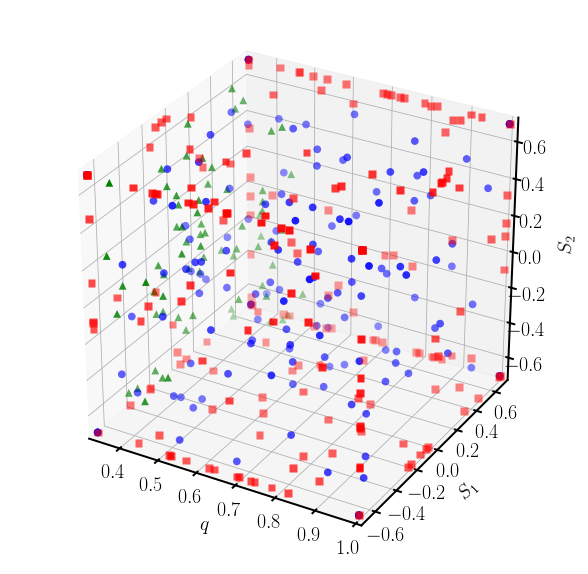
\includegraphics[width=0.49\textwidth]{trainingset3d.png}\\
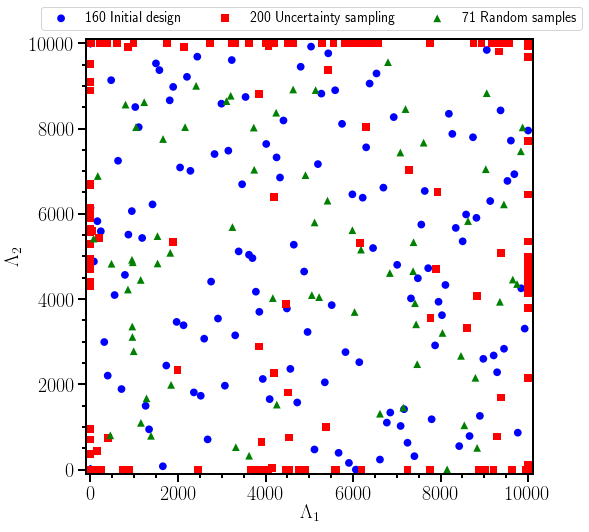
\includegraphics[width=0.49\textwidth]{trainingset2d.png}
\caption{Projection of the sampled waveforms onto the three-dimensional subspace $\{q, S_1, S_2\}$ (top)
and the two-dimensional subspace $\{\Lambda_1, \Lambda_2\}$ (bottom). The 160 black circles were used for the initial
training set (32 corner points + 128 LHD points) that generated the initial surrogate. The 200 red squares were generated
using uncertainty sampling from the GPR error estimate of the RMS phase error at the empirical nodes. 
}
\label{fig:LHD}
\end{figure}

\subsection{Conditioning and decomposing the training set waveforms}

--Messy details of preconditioning lalsimulation waveforms to make them smooth functions of parameters ${\bm x}$.
(Rescale with total mass to convert to geometric units, time shift to align at max amplitude or specific frequency, 
taper beginning and end, pad end with zeros, Fourier transform, truncation, resampling, zeroing initial phase, ...)

--Show plot (?) to validate that waveform is properly conditioned by plotting amplitude/phase as function of waveform parameters
at specific frequencies and show that they're smooth functions.

\begin{equation}
\tilde h(f, x) = A(f, x) e^{i\Phi(f, x)}
\end{equation}

Because the waveform $h$ is an oscillatory function of $f$ and ${\bm x}$ that is difficult to interpolate, we instead construct 
surrogates for the amplitude $A(f, x)$ and phase $\Phi(f, x)$. These are smooth functions. However, for aligned-spin waveforms
these functions are already approximately known from the 3.5PN TaylorF2 waveform 
$\tilde h_{\rm F2}(f, x) = A_{\rm F2}(f, x) e^{i\Phi_{\rm F2} (f, x)}$, where
\begin{equation}
A_{\rm F2} = simple equation,
\end{equation}
and
\begin{equation}
\Phi_{\rm F2} = not simple equation.
\end{equation}
We therefore only have to construct surrogates for the difference between EOB and TaylorF2:
\begin{align}
\Delta\ln(A) &= \ln(A/A_{\rm F2})\\
\Delta\Phi & = \Phi - \Phi_{\rm F2}
\end{align}
These quantities are shown in Fig.~\ref{fig:dh} for the training set wavefroms. We note that for small differences 
between the EOB and TaylorF2 waveform, $\Delta\ln A$ is approximately the fractional difference $A/A_{\rm F2} - 1$
between the EOB and TaylorF2 waveform. We use the log-ratio instead of the ratio, because it guarantees that any
error in interpolating this quantity doesn't result in a negative amplitude. Also, because waveforms tend to deviate from 
each other near the end of the inspiral exponentially, depending on each waveform's merger frequency the log captures
this behavior. [[Is this true for EOB? We'll find out.]]

\begin{figure}[htb]
\centering
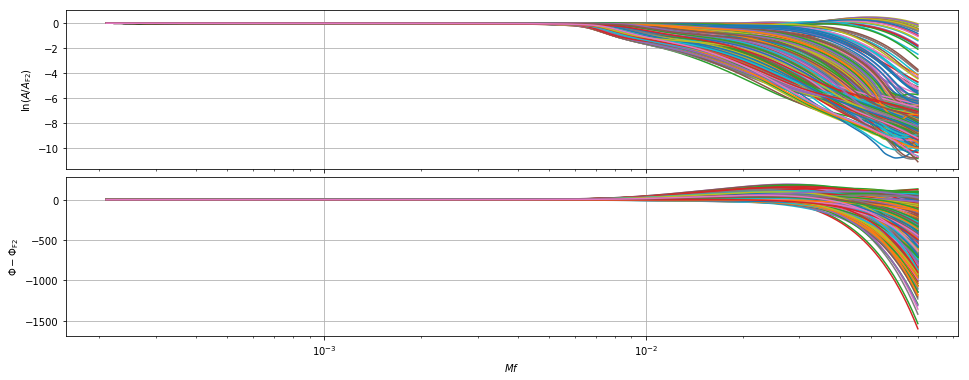
\includegraphics[width=0.49\textwidth]{dh_trainingset.png}
\caption{Training set}
\label{fig:dh}
\end{figure}

We show the range of values of the phase $\Phi$ over the training set $\Phi_{\rm range} = \Phi_{\rm max} - \Phi_{\rm min}$ 
as well as the range of values of the phase residual $\Delta\Phi$ over the training set 
$\Delta\Phi_{\rm range} = \Delta\Phi_{\rm max}-\Delta\Phi_{\rm min}$ in Fig.~\ref{fig:phaserange}. 
The range in $\Phi$ can be larger than 1000~radians, meaning
that if we require 0.1~radian accuracy, we need a fractional error of $<10^{-4}$. The range of $\Delta\Phi$ is 1--2 orders 
of magnitude smaller, and as a result, the interpolation accuracy requirements are 1--2 orders of magnitude smaller as well. 

\begin{figure}[htb]
\centering
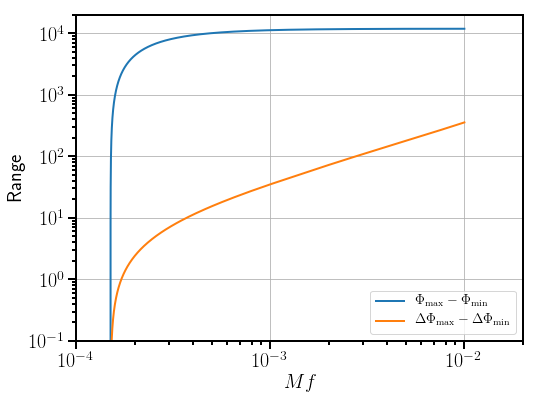
\includegraphics[width=0.49\textwidth]{phaserange.png}
\caption{Range of phase values for training set waveforms. The range is a factor of $\gtrsim 100$ larger for $\Phi$ than for $\Delta\Phi$, 
meaning that the interpolation accuracy requirements are at least $\sim 2$ orders of magnitude less for $\Delta\Phi$.}
\label{fig:phaserange}
\end{figure}


\subsection{Compression of waveform data with reduced bases and empirical interpolation method}

For many surrogate problems a function $f({\bm x})$ is sought to interpolate a scalar quantity $y$. For the
problem here, the outputs are the quantities $\Delta\ln A$ and $\Delta\Phi$ sampled at the frequencies $f_j$. 
One could interpolate $\Delta\ln A$ and $\Delta\Phi$ as a function of ${\bm x}$ at each sample $f_j$, 
however, this would be prohibitively expensive. Instead we use the standard method of constructing an
orthonormal reduced basis to compress each training set waveform into a small set of coefficients, 
and then using the empirical interpolation method
to optimize the placement of a corresponding number of empirical nodes $F^A_j$ and $F^\Phi_j$. One then interpolates
$\Delta\ln A$ and $\Delta\Phi$ as a function of ${\bm x}$ at these nodes. The full waveform can then be reconstructed by 
multiplying the value at these nodes by the the corresponding empirical interpolating functions $B_j^A(f)$ and $B_j^\Phi(f)$. 
The methods used here are presented in Refs.[[cite]], and we use the exact implementation described in 
Ref.~[[LackeyBernuzziGalley2017]]. We briefly describe the details.

In order to construct a reduced basis from the training set waveforms we use the greedy method~[[LackeyBernuzziGalley2017]
to choose a subset of the training set waveforms and orthonormalize them with the Grahm-Schmidt procedure. The end result
is similar to singular value decomposition, but one can make a one-to-one mapping between each chosen waveform and a 
corresponding basis function. The quantities $\Delta\ln A$ and $\Delta\Phi$ can be approximately described by
\begin{subequations}
\label{eq:basis1}
\begin{align}
\Delta\ln A(f; \btheta) \approx {} & \sum_{i=1}^{N_A} e^A_i(f) c^A_i(\btheta)\\
\Delta\Phi(f; \btheta) \approx {} & \sum_{i=1}^{N_\Phi} e^\Phi_i(f) c^\Phi_i(\btheta),
\end{align}
\end{subequations}
where the coefficients are
\begin{subequations}
\label{eq:basiscoeffs1}
\begin{align}
c_i^A(\btheta) & = \langle e_i^A(\cdot) , \Delta\ln A(\cdot; \btheta) \rangle \\
c_i^\Phi(\btheta) & = \langle e_i^\Phi(\cdot) , \Delta\Phi(\cdot; \btheta) \rangle  .
\end{align}
\end{subequations}

In the empirical interpolation method, one chooses a set of frequencies $F_j$ [[to ... minimize impact of interpolation error]].
The reduced basis can then be inverted to construct empirical interpolating functions $B_j(f)$ [[details...]].
\begin{subequations}
\label{eq:empinterpFinal}
\begin{align}
\Delta\ln A_S(f; \btheta ) & = \sum_{j=1}^{N_A} B_j^A(f) \Delta\ln A(F^A_j; \btheta) \\
\Delta\Phi_S(f; \btheta ) & = \sum_{j=1}^{N_\Phi} B_j^\Phi(f) \Delta\Phi(F^\Phi_j; \btheta)
\end{align}
\end{subequations}
The interpolating functions for $\Delta\ln A$ and $\Delta\Phi$ are shown in Fig.~\ref{fig:B}. 

\begin{figure}[htb]
\centering
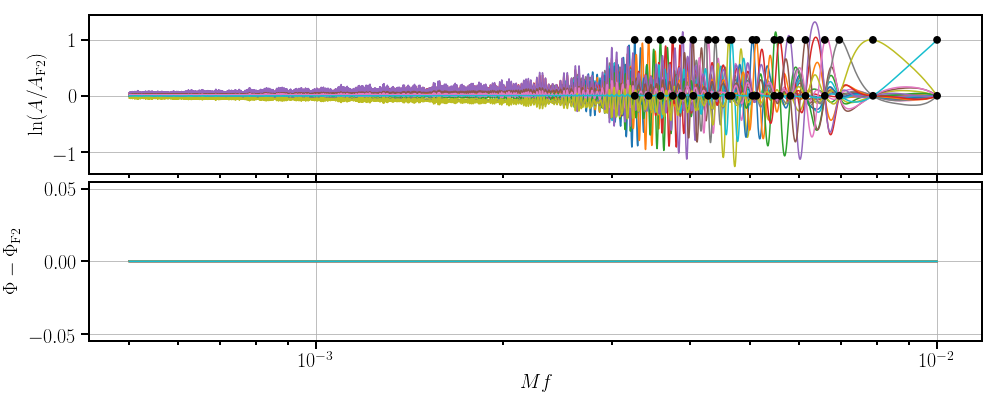
\includegraphics[width=0.49\textwidth]{Bamp.png}
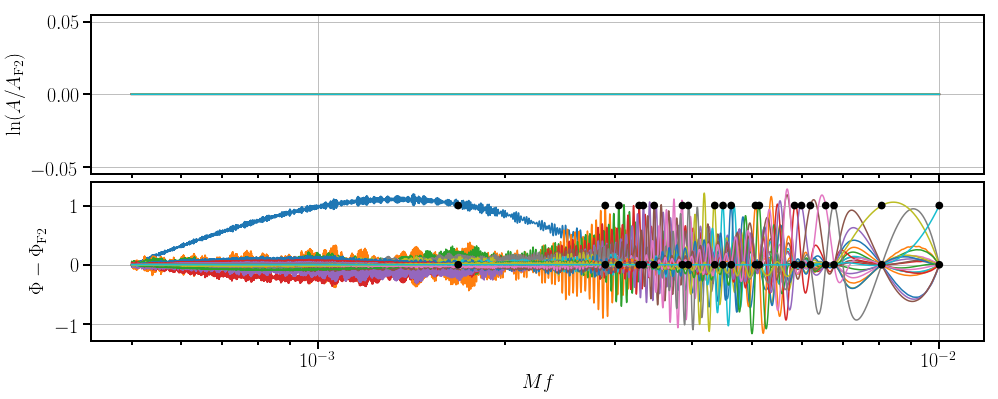
\includegraphics[width=0.49\textwidth]{Bphase.png}
\caption{Top: $B^{\rm Amp}_j(Mf)$. Bottom: $B^{\rm Phase}_j(Mf)$. Black dots indicate the frequency of the empirical nodes $MF_j$.}
\label{fig:B}
\end{figure}

\subsection{Interpolating over waveform parameter space}

We use Gaussian process regression to fit $\Delta\ln A$ and $\Delta\Phi$ at the empirical nodes as a function of
the waveform parameters. In GPR a function $f(\vec x)$ is described in terms of a mean $m(\vec x)$ and 
covariance $k(\vec x, \vec x')$ between points [[cite RassmussenWilliamsChapter2, IntroArxivPaper]].
\begin{equation}
f(\vec x) \approx \mathcal{GP}(m(\vec x), k(\vec x, \vec x')).
\end{equation}
The mean $m(x)$ can be some parameterized function which is the standard version of regression, 
while $k(\vec x, \vec x')$ is a kernel with tunable hyperparameters that describes the covariance between
the point $\vec x$ and the sampled point $\vec x'$. This covariance can be used to describe features of the function 
not captured by the parameterized mean as well as genuine noise in the data ${\bm y}$. 
For the problem here, we have already subtracted the 
TaylorF2 waveform from EOB waveform, so we set $m=0$ and model the remainder terms purely in terms 
of the covariance $k$. 

In a zero-mean Gaussian process, the data and function $({\bm y}, f_*)$ at the training set and new points $({\bm x}, x_*)$ are
drawn from a multivariate normal distribution
\begin{equation}
\label{eq:gaussian}
\begin{bmatrix}
{\bm y} \\
f_* \\
\end{bmatrix}
\sim \mathcal{N}
\left({\bm 0}, 
\begin{bmatrix}
K & K_*^T \\
K_* & K_{**} \\
\end{bmatrix}
\right)
\end{equation}
where $K = K({\bm x}^i, {\bm x}^j)$ is a matrix, $K_* = K({\bm x}^i, {\bm x}_*)$ is a vector, and $K_{**} = K({\bm x}_*, {\bm x}_*)$ is a scalar.

The conditional probability for $f_*$ given the training set examples ${\bm y}$ with hyperparameters $\theta$ is also a Gaussian
\begin{equation}
f_* | {\bm x}, x_*, {\bm y}, {\bm \theta} \sim \mathcal{N}(\bar f_*, {\rm var}(f_*))
\end{equation}
where the mean and variance are
\begin{align}
\label{eq:mean}
\bar f_* &= K_*^T K^{-1} y \\
\label{eq:var}
{\rm var}(f_*) &= K_{**} - K_*^T K^{-1} K_*.
\end{align}
Eq.~\eqref{eq:mean} is the estimate of the function, and Eq.~\eqref{eq:var} is the estimate of the uncertainty, where we note that the variance does not depend on the data $\bm{y}$.

We use a radial kernel which expresses the covariance in terms of a distance $r$ between points
\begin{equation}
r^2 = (x-x')^T M (x-x'),
\end{equation}
where we choose the matrix M to be diagonal
\begin{equation}
M = {\rm diag}(\ell_1^{-2}, \ell_2^{-2}, \dots, \ell_d^{-2}).
\end{equation}
The tunable hyperparameters $\ell_i$ represent the length scale over which the function $f(x)$ varies in 
each coordinate $x_i$. Specifically, we use the Mat\'{e}rn class of kernels
\begin{equation}
k_{\rm Matern}(r) = \frac{2^{1-\nu}}{\Gamma(\nu)} \left(\sqrt{2\nu} r\right)^\nu K_\nu \left(\sqrt{2\nu} r \right).
\end{equation}
where $K_\nu(x)$ is a modified Bessel function. The value of $\nu$ parameterizes the smoothness of the 
Gaussian Process $f(x)$, and is $k$ times mean-square differentiable if $\nu>k$ [[cite]]. For half-integer values of $\nu$, this 
kernel has a computationally cheap form without special functions, and we have had good results with $\nu=5/2$, 
resulting in a twice-differentiable function. The $\nu=5/2$ kernel is
\begin{equation}
k_{\rm Matern}^{\nu=5/2}(r) = \left(1+\sqrt{5}r + \frac{5r^2}{3}\right) \exp\left(-\sqrt{5}r\right).
\end{equation}

Our final kernel takes the form
\begin{equation}
k(x_p, x_q) = \sigma_f^2 k_{\rm Matern}^{\nu=5/2}(r) + \sigma_n^2 \delta_{pq}
\end{equation}
where $\sigma_f$ is a scale factor that describes the range of values that $f(x)$ takes over the domain, 
and $\sigma_n$ is a noise parameter. The white noise kernel $\sigma_n^2 \delta_{pq}$ (also called a nugget), which is
$\sigma_n^2$ when $x_p=x_q$ and zero otherwise, is generically used for numerical stability, but also parameterizes
noise in the data ${\bm y}$. In our case, the training set waveforms which are evaluated, tapered, and 
Fourier transformed numerically have numerical noise that we will estimate by optimizing the hyperparameters.
The hyperparameters now are $\theta = \{\sigma_f, \ell_q, \ell_{S_1}, \ell_{S_2}, \ell_{\Lambda_1}, \ell_{\Lambda_2}, \sigma_n\}$.

[[In principle, one can select the optimal class of kernels using k-fold or leave-one-out cross validation. We have also tried the 
more common infinitely differentiable squared exponential kernel. However, we found it difficult to reliably tune the 
hyperparameters for the problem here.]]

In order to estimate the hyperparameters, we use the above assumption (Eq.~\eqref{eq:gaussian}) that the joint distribution of 
the data ${\bm y}$ is a multivariate Gaussian which has the following distribution
\begin{equation}
\ln p({\bm y} | {\bm x}, {\bm \theta}) = -\frac{1}{2}{\bm y}^T K^{-1} {\bm y} - \frac{1}{2} \ln |K| - \frac{d}{2} \ln 2\pi.
\end{equation}
This is the log-likelihood for ${\bm y}$ given the hyperparameters ${\bm \theta}$, and we can find the posterior for ${\bm \theta}$
given ${\bm y}$ using Bayes' theorem
\begin{equation}
p({\bm \theta} | {\bm x}, {\bm y}) \propto p({\bm \theta}) p({\bm y} | {\bm x}, {\bm \theta}).
\end{equation}
The prior $p({\bm \theta})$ is typically uniform and used to set the bounds on ${\bm \theta}$. If interested in the distribution of the 
hyperparamaters, one can sample this posterior with, for example, Markov chain Monte Carlo. However, for the problem here, we are
simply interested in finding the maximum of the posterior. To do this, we use the \texttt{gaussian\_process} module in the
\texttt{scikit-learn} package [[cite]]. Finally, with the optimized hyperparameters ${\bm \theta}$, Eq.~\eqref{eq:var} is the 
interpolating function. We note that evaluating Eq.~\eqref{eq:var}, is an $\mathcal{O}(N)$ operation if the vector $K^{-1}{\bm y}$ is
precomputed.




\subsection{Choosing new training set waveforms}

Once we have an initial surrogate model, we can choose new training set samples by iteratively searching the parameter space
for new points ${\bm x}$ that maximize some error criterion. The quantity that we use is the distinguishability between the
EOB waveform and its surrogate [[cite]]
\begin{equation}
|\delta h | = \sqrt{(h - h_{\rm Sur} | h - h_{\rm Sur})}.
\end{equation}
For an initial training set with N samples, this function has $\sim N$ local maxima. We use Monte Carlo sampling with ~100,000
samples and choose the point with the largest distinguishability [[for now. Could also use multistart optimization.]] to find the 
approximate global maximum. Because $|\delta h |$ is an expensive function that requires an EOB or NR evaluation, 
we approximate it as follows:

[[Your inexpensive way of approximating $|\delta h |$ that does not depend on $h_{\rm EOB}$ here.]]
\begin{equation}
\label{eq:distinguish}
|\delta h | \approx blah.
\end{equation}


With this new sample, one could evaluate the waveform at the new point and reconstruct the surrogate model, then iterate.

Reconstructing the surrogate for each new sample is inexpensive compared to the time needed to simulate a new NR waveform. 
However, even for NR waveforms, one often wants to perform $N_{\rm new}$ new waveform simulations in parallel. 
We therefore need a method for optimally choosing $N_{\rm new}$ new samples. One could simply choose the 
$N_{\rm new}$ local maxima with the largest $|\delta h |$. However, there is a more optimal way of iteratively finding new points.
If we hold the hyperparameters ${\bm \theta}$ fixed, we note that the GPR error estimate (Eq.~\eqref{eq:var}) does not depend
on the data ${\bm y}$, just on the samples ${\bm x}$. Therefore, the approximate $|\delta h |$ (Eq.~\eqref{eq:distinguish}) does not depend
on the new samples either. The method uses the idea of uncertainty sampling [[cite]] but without updating the hyperparameters
after each new point is chosen. The algorithm for choosing the new points is as follows.

While $|\delta h |_{\rm max} > \epsilon$:
\begin{enumerate}
\item Construct the GPR error functions (Eq.~\eqref{eq:var}) at each of the empirical nodes $F^A_j$ and $F^\Phi_j$.
In practice this can be done by specifying the samples ${\bm x}$, the hyperparameters ${\bm \theta}$, and dummy 
data ${\bm y}={\bm 1}$. These GPR error functions are the input to Eq.~\eqref{eq:distinguish}.

\item Find $({\bm x}_{\rm max}, |\delta h |_{\rm max})$ that maximizes Eq.~\eqref{eq:distinguish} over the parameter space. 
\item Add ${\bm x}_{\rm max}$ to the list of samples: ${\bm x} = [{\bm x}, {\bm x}_{\rm max}]$.
\end{enumerate}
These new waveforms can now be evaluated in parallel.

[[The methods used here fall under the terms active learning and Bayesian optimization [[cite]]. The specific method being used is
uncertainty sampling [[cite]]. The parallelization method I am using I have not seen in the literature. Is it actually new? Ask Niki.]]


[[Another method you could try is k-means clustering of the mismatch for your validation set (using mismatch above some threshold), 
where you have $k=N$, because there will
be $\sim N$ local maxima of the mismatch. Within each cluster, choose the waveform with the largest mismatch and add it to the
training set. This way you only use one new point per local maximum region. You could do the same thing with the Fisher matrix
systematic error calculation instead of the mismatch if that's a better quantity to use.]]

\begin{figure}[htb]
\centering
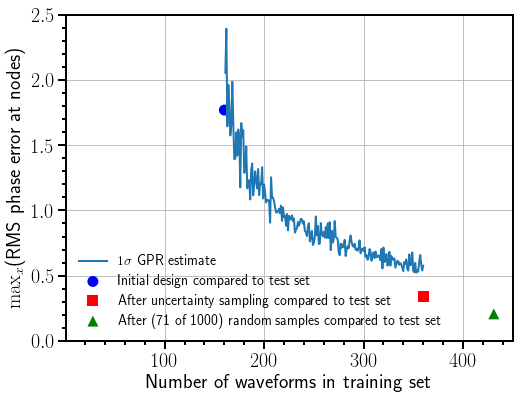
\includegraphics[width=0.49\textwidth]{uncertaintysampling.png}
\caption{Estimated RMS phase error as function of number of sampled points}
\label{fig:phaserange}
\end{figure}


\subsection{Surrogate waveform evaluation}

--Constructing the final model with units, inclination angle, time and phase shift, etc.

--Implementation details


%% ________________________________________________________
\section{Results}

\subsection{Accuracy}

--Phase error. (needs to be significantly smaller than tidal effects) Use this for order of magnitude estimate of required
accuracy.

\begin{figure}[htb]
\centering
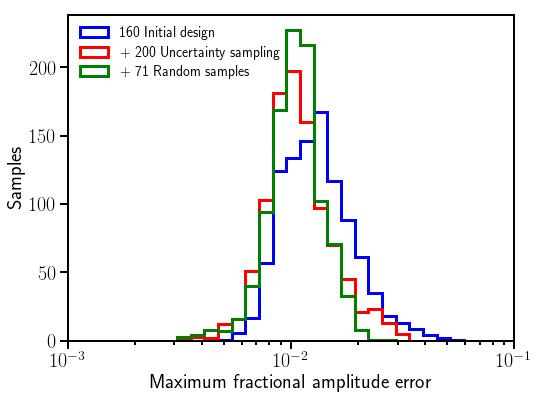
\includegraphics[width=0.49\textwidth]{maxamphist.png}
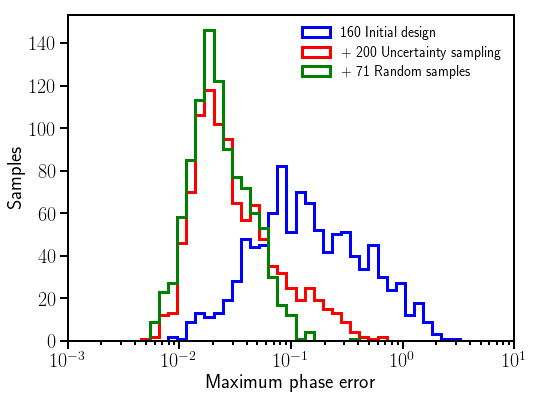
\includegraphics[width=0.49\textwidth]{maxphasehist.png}
\caption{Amplitude and phase error.}
\label{fig:phaserange}
\end{figure}

\begin{figure}[htb]
\centering
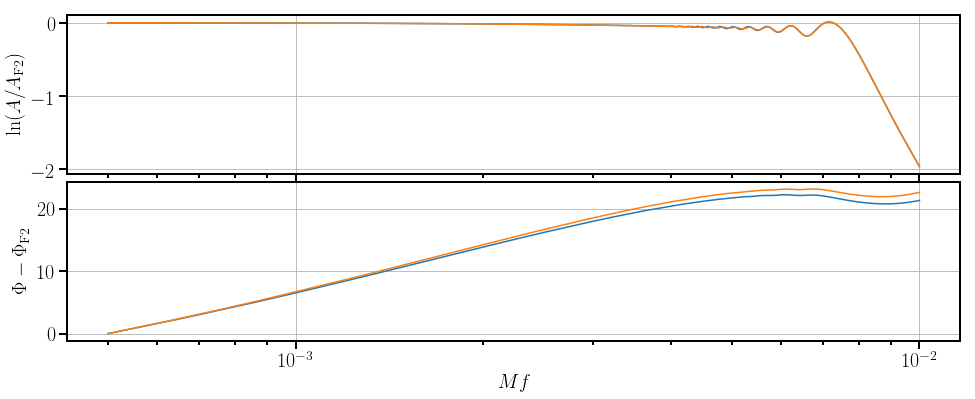
\includegraphics[width=0.49\textwidth]{dhmaxerror.png}
\caption{Waveform with largest phase error. It's parameters are....}
\label{fig:phaserange}
\end{figure}


In Fig.~\ref{fig:mismatch}, we show the distribution of mismatch $\mathcal{M}$ between our surrogate
and the $10^4$ randomly sampled EOB waveforms. We use the design sensitivity aLIGO PSD~\cite{Aasi:2013wya} and
a sampling rate of 4096~Hz. Our integration bounds are $f_{\rm low} = x$~Hz and the Nyquist frequency
$f_{\rm high} = 2048$~Hz. Because the surrogate can be rescaled with mass,
we show results for the smaller mass $M_B$ fixed at $1M_\odot$ or fixed at $2M_\odot$.
We also show the mismatch as a function of parameters in Fig.~\ref{fig:mismatchtriangle}.
It is generally largest for as the mass ratio decreases toward $1/3$.


\begin{figure}[htb]
\centering
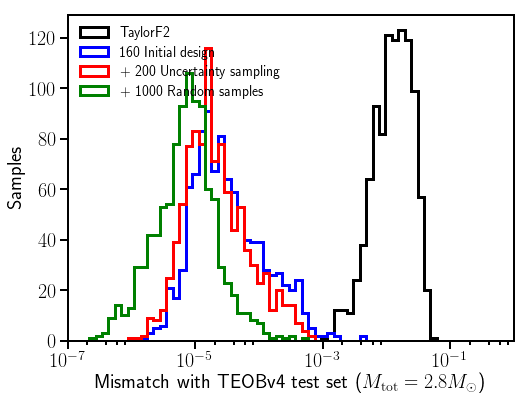
\includegraphics[width=0.49\textwidth]{mismatch.png}
\caption{Mismatch. \red{[[You should do mismatch with TaylorF2 as a reference for the improvement in 
going through all the effort in this paper.]]}
}
\label{fig:mismatch}
\end{figure}

\begin{figure}[htb]
\centering
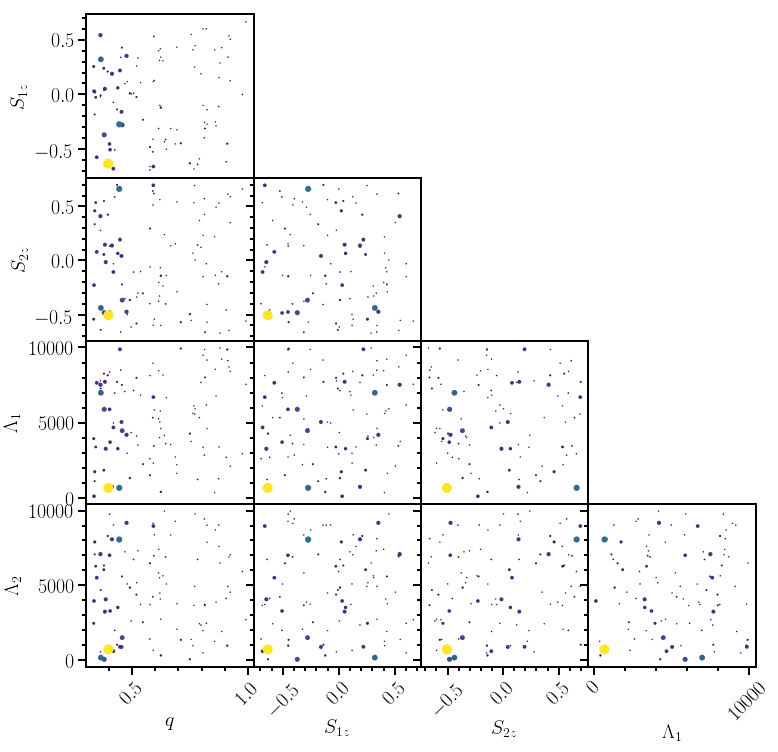
\includegraphics[width=0.49\textwidth]{mismatchtrianglem10.png}
\caption{Mismatch for systems with $m_2=1M_\odot$.}
\label{fig:mismatchtriangle}
\end{figure}


--distinguishability

--Fisher matrix systematic error.



\subsection{Timing}

Although optimizing the hyperparameters scales with number of samples $n$ as $\mathcal{O}(n^3)$
due to the required matrix inversion, the evaluation time of a stored GPR scales as $\mathcal{O}(n)$.
The evaluation time for the waveform functions will therefore be $\mathcal{O}(n(N_A+N_\Phi))$.

The surrogate has a fixed time of $\sim 50$~ms to evaluate the GPR at each node then evaluate the amplitude
and phase at the log-spaced frequencies. Then, there is an additional cost to resample the amplitude and phase
at uniformly-spaced frequencies with interpolation, and finally evaluating $\tilde h_+$ and $\tilde h_\times$. 
Below 50~Hz the surrogate is faster than all models except TaylorF2 [[you didn't try PhenomP etc.]], and below
18~Hz it is faster than TaylorF2. 

\begin{figure}[htb]
\centering
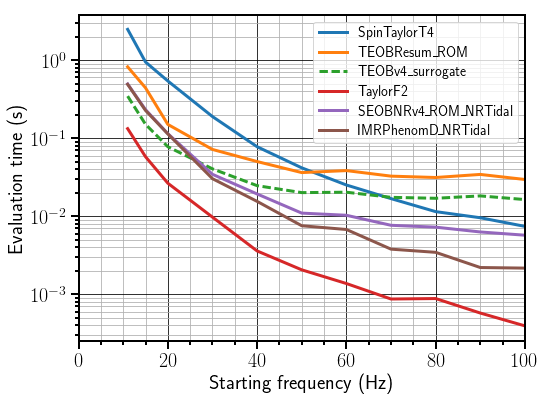
\includegraphics[width=0.49\textwidth]{timing.png}
\caption{Waveform evaluation time as a function of the waveform starting frequency. The time-domain waveforms
were sampled at 4096~Hz then Fourier transformed. The frequency-domain waveforms used the
same frequency samples as the Fourier transformed time-domain waveforms.}
\label{fig:timing}
\end{figure}

--Frequency domain allows for evaluating likelihood with non-uniform sampling.

--Can construct a ROQ of the model if needed.

\subsection{Parameter estimation}

--Can only include this section if there's a LAL version. Should you bother?


\section{Discussion}

\subsection{Review}



\subsection{Future work}

Hierarchical method and uncertainty sampling provides way to construct surrogate from minimal number of waveforms.

--Could be used to correct the very end of inspiral (and post-merger) with NR simulations where only O(100) simulations are feasable.


%% ________________________________________________________
\begin{acknowledgments}

BL thanks... BL was supported by... 

\end{acknowledgments}


%% ________________________________________________________
%\bibliographystyle{revtex}     
\bibliography{paper,refs}  


\end{document}

\begin{widetext}
\begin{align}
\Lambda_{2,\textrm{dyn}}^{\textrm{(A,B)}}(u) = &\frac{\lambda_{2}^{\textrm{(1,2)}}}{M^5} \left\{\frac{1}{4} + \frac{3}{4} \left(\frac{\omega^{(1,2)}_{f,2}}{2\Omega}\right)^2\left[\frac{4\Omega^2}{(\omega^{(1,2)}_{f,2})^2 - 4\Omega^2} + \frac{10}{3Q}\right.\right. \nonumber\\
&\left.\left.+\sqrt{\frac{\pi}{3}}\frac{1}{\epsilon_{1,2}}\left[(1 + 2\mathcal{S}{(y_{1,2})})\cos{\left(\frac{\pi}{2}y^2_{1,2}\right)} - (1 + 2\mathcal{C}{(y_{1,2})})\sin{\left(\frac{\pi}{2}y_{1,2}^2\right)}\right]\right]\right\}\,,\\
\Lambda_{3,\textrm{eff}}^{\textrm{(1,2)}} (u)= &\frac{\lambda_{3}^{\textrm{(1,2)}}}{M^7} \left\{\frac{3}{8} + \frac{(\omega^{(1,2)}_{f,3})^2}{\Omega^2}\left(\frac{25}{48 O_{1,2}} + \frac{5}{72}\frac{9\Omega^2}{(\omega^{(1,2)}_{f,3})^2-9\Omega^2}\right)\right. \nonumber\\
&\left.+ O_{1,2}\left[\cos{(w^2)}\left(\frac{1}{2} +\mathcal{S}(sqrt2pi*w)\right) - \sin{(w^2)}\left(\frac{1}{2} + \mathcal{C}(sqrt2pi*w)\right)\right]\right\}\,,
\end{align}
\end{widetext}
where $\lambda_{2}^{\textrm{(1,2)}}$ are the (constant) adiabatic values of the quadrupolar tidal polarizabilities, $\lambda_{3}^{\textrm{(1,2)}}$ are the (constant) adiabatic values of the octupolar tidal polarizabilities, $\omega^{(1,2)}_{f,2}$ are the quadrupolar $f$-mode frequencies, $\omega^{(1,2)}_{f,3}$ are the octupolar $f$-mode frequencies, $\mathcal{S}$ is the Fresnel sine integral, $\mathcal{C}$ is the Fresnel cosine integral, $\epsilon_{1,2} = 2^{19/3}\nu (M\omega^{(1,2)}_{f,2})^{5/3}/5$,   $y_{1,2}=\sqrt{3/(\pi \epsilon)} Q_{1,2}/5$, and $Q_{1,2} = 4- 2^{1/3}(M\omega^{(1,2)}_{f,2})^{5/3}u^{-5/2}$. 
, $w_{1,2}=O_{1,2}/(4\,3^{2/3}\sqrt{10}(M\omega^{(1,2)}_{f,3})^{5/6}\sqrt{\nu})$, $O_{1,2}=5\sqrt{5\pi}/u^3(M\omega^{(1,2)}_{f,3})^{7/6}/(192\,3^{2/3}\sqrt{\nu})$.

